\documentclass{article}
\usepackage{tikz}

\begin{document}

\begin{figure}[h]
    \centering
    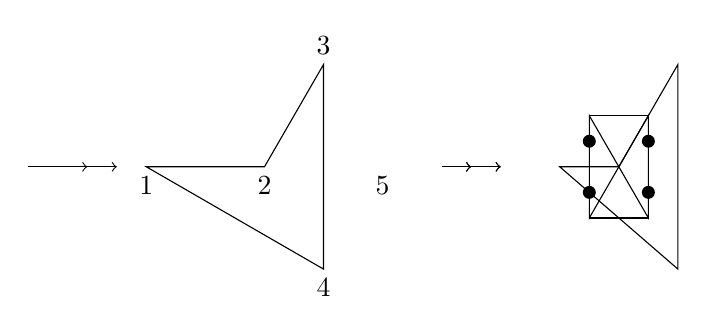
\begin{tikzpicture}[scale=1.5]
        % Define coordinates for the vertices
        \coordinate (A) at (0,0);
        \coordinate (B) at (1,0);
        \coordinate (C) at (1.5,0.866);
        \coordinate (D) at (1.5,-0.866);
        \coordinate (E) at (2,0);
        
        % Draw the initial diamond shape
        \draw (A) -- (B) -- (C) -- (D) -- cycle;
        
        % Label the vertices
        \node at (A) [below] {$1$};
        \node at (B) [below] {$2$};
        \node at (C) [above] {$3$};
        \node at (D) [below] {$4$};
        \node at (E) [below] {$5$};
        
        % Draw the arrows indicating the replacement rule
        \draw[->] (-1,0) -- (-0.5,0);
        \draw[->] (-0.5,0) -- (-0.25,0);
        \draw[->] (2.5,0) -- (2.75,0);
        \draw[->] (2.75,0) -- (3,0);
        
        % Define coordinates for the second step of the replacement
        \coordinate (F) at (3.5,0);
        \coordinate (G) at (4,0);
        \coordinate (H) at (4.5,0.866);
        \coordinate (I) at (4.5,-0.866);
        \coordinate (J) at (5,0);
        
        % Draw the second diamond shape
        \draw (F) -- (G) -- (H) -- (I) -- cycle;
        
        % Define coordinates for the smaller diamonds
        \coordinate (K) at (3.75,0.433);
        \coordinate (L) at (3.75,-0.433);
        \coordinate (M) at (4.25,0.433);
        \coordinate (N) at (4.25,-0.433);
        
        % Draw the smaller diamonds
        \draw (K) -- (L) -- (M) -- (N) -- cycle;
        \draw (K) -- (M) -- (N) -- (L) -- cycle;
        
        % Define coordinates for the smaller triangles
        \coordinate (O) at (3.75,0);
        \coordinate (P) at (4.25,0);
        
        % Draw the smaller triangles
        \draw (O) -- (K) -- (L) -- cycle;
        \draw (P) -- (M) -- (N) -- cycle;
        
        % Define coordinates for the smaller circles
        \coordinate (Q) at (3.75,0.2165);
        \coordinate (R) at (3.75,-0.2165);
        \coordinate (S) at (4.25,0.2165);
        \coordinate (T) at (4.25,-0.2165);
        
        % Draw the smaller circles
        \filldraw (Q) circle (0.05);
        \filldraw (R) circle (0.05);
        \filldraw (S) circle (0.05);
        \filldraw (T) circle (0.05);
        
        % Draw the arrows indicating the replacement rule for the second step
        \draw[->] (2.5,0) -- (2.75,0);
        \draw[->] (2.75,0) -- (3,0);
    \end{tikzpicture}
    \caption{Figure of a symmetric replacement rule that produces the ``Laakso diamond'' space that first appeared in \cite{Laakso}, and was studied e.g. in \cite{Yair, LangPlaut}. The figure shows two steps of the replacement.}
    \label{fig:laakso_diamond}
\end{figure}

\end{document}